\documentclass[conference]{IEEEtran}
\IEEEoverridecommandlockouts

\usepackage[utf8]{inputenc}
\usepackage[T2A]{fontenc}
\usepackage[russian]{babel}
\usepackage{cite}
\usepackage{amsmath,amssymb,amsfonts,amsthm}
\usepackage{algorithmic}
\usepackage{graphicx}
\usepackage{textcomp}
\usepackage{xcolor}
\usepackage{booktabs}

\theoremstyle{plain}
\newtheorem{proposition}{Утверждение}
\newtheorem{lemma}{Лемма}
\theoremstyle{definition}
\newtheorem{remark}{Замечание}
\newtheorem{definition}{Определение}
\newtheorem{hypothesis}{Гипотеза}

\newcommand{\R}{\mathbb{R}}
\newcommand{\E}{\mathbb{E}}
\newcommand{\norm}[1]{\left\lVert#1\right\rVert}
\newcommand{\Sstable}{\mathcal{S}_\alpha}
\DeclareMathOperator*{\argmin}{arg\,min}
\DeclareMathOperator{\med}{med}
\DeclareMathOperator{\Var}{Var}
\DeclareMathOperator{\sgn}{sgn}

\begin{document}

\title{Шумоподавление наблюдаемого ряда как предобработка\\
стохастической оптимизации: когда фильтрация спасает\\
сходимость при тяжёлохвостовом градиентном шуме}

\author{%
\IEEEauthorblockN{Дмитрий Кортунов}
\IEEEauthorblockA{\textit{НИУ ВШЭ}\\ Москва, Россия}
\and
\IEEEauthorblockN{Вадим Пастушенко}
\IEEEauthorblockA{\textit{НИУ ВШЭ}\\ Москва, Россия}
\and
\IEEEauthorblockN{Алексей Дубовицкий}
\IEEEauthorblockA{\textit{НИУ ВШЭ}\\ Москва, Россия}
\and
\IEEEauthorblockN{Андрей Шадрин}
\IEEEauthorblockA{\textit{НИУ ВШЭ}\\ Москва, Россия}
}

\maketitle

\begin{abstract}
Шумоподавление наблюдаемого ряда трактуется как явный этап
конвейера стохастической оптимизации. Сначала формализуется модель
временного ряда и задача прогноза (раздел II), затем выносится
теоретический фон с механизмом эффекта и гипотезами (раздел III), затем
описывается экспериментальная проверка (раздел IV) и, наконец,
эмпирически обоснованные практические критерии выбора связки
``фильтр+оптимизатор'' (раздел V). Главный механизм: при
$\alpha$-устойчивом градиентном шуме ($\alpha<2$, бесконечная
дисперсия) SGD с постоянным шагом не имеет конечного шумового пола;
оконная медиана отображает окно с бесконечной дисперсией в порядковую
статистику с конечной дисперсией, что восстанавливает стандартный пол,
тогда как любой \emph{линейный} фильтр (скользящее среднее, Калман)
сохраняет $\alpha$-устойчивый закон. Для смешанного режима
(тяжёлые хвосты + долгая память) одиночная медиана уже не работает ---
вводится \emph{причинный каскадный фильтр} $F_{10}$ (медиана $\to$
Калман) и его адаптивная версия $F_{11}$ (стадии выбираются по
$\hat\alpha,\hat H$), которые мы предлагаем именно для этого режима.
Эмпирически при $\hat\alpha\approx1.2$ обычный SGD сходится в $0/8$
прогонах (как и линейные/вейвлет-фильтры) и в $8/8$ с причинной
медианой, снижая пол в $108\times$ (квадратичная) и $133\times$
(логистическая); эффект сохраняется при калибровке ($91\times$/$120\times$)
и подтверждён на расширенной корзине реальных доменов (финансовые
дневные/15-минутные/5-минутные, FRED, ETTh1, ETTh2, ETTm1, sunspots) с
обоих сторон --- и где фильтрация ускоряет ($\approx78\times$ на 15-мин),
и где не помогает (чистый гаусс, долгопамятные смеси).
\end{abstract}

\begin{IEEEkeywords}
стохастическая оптимизация, тяжёлохвостовый шум, $\alpha$-устойчивые
распределения, медианная фильтрация, причинный каскадный фильтр,
фильтр Калмана, долгая память, сходимость.
\end{IEEEkeywords}

% ============================================================
\section{Введение}
% ============================================================

Теория сходимости стохастических методов первого порядка опирается на
конечный второй момент градиентного шума и слабую временную зависимость.
Оба предположения нарушаются при обучении на финансовых рядах:
доходности тяжёлохвостовы и долгопамятны
\cite{cont2001,mandelbrot1963}, и стохастический градиент
наследует эти свойства \cite{simsekli2019tailindex}. Мы рассматриваем
шумоподавление не как визуализацию, а как вычислительный этап между
наблюдениями и оптимизатором, и ставим точный вопрос: для каких троек
(шум, фильтр, оптимизатор) предобработка превращает несходящийся
прогон в сходящийся и почему.

Структура текста задана по разделам:
\textbf{II}~--- модель временного ряда, термины, задача прогноза и
формальная постановка решаемой задачи (\emph{без} описания алгоритмов);
\textbf{III}~--- теоретический фон и явно сформулированные гипотезы
(\emph{с} компактными определениями фильтров и оптимизаторов как
аналитических объектов);
\textbf{IV}~--- экспериментальный план, расширенная корзина реальных
доменов (включая нефинансовые) и анализ;
\textbf{V}~--- практические критерии выбора, где каждый пункт явно
помечен как ``из теории'', ``из эксперимента'' или ``эвристика'';
\textbf{VI}~--- заключение.

\textbf{Вклад статьи.} (i)~Чистая формализация задачи, отделённая от
конкретных алгоритмов; (ii)~утверждение, выделяющее механизм:
нелинейная порядковая статистика восстанавливает конечную эффективную
дисперсию шума, чего линейные фильтры дать не могут;
(iii)~\emph{новый причинный каскадный фильтр} $F_{10}$ и его адаптивный
вариант $F_{11}$, спроектированные под предсказанный негативный режим
N4 (тяжёлые хвосты $\cap$ долгая память); вместе с медианой $F_4$ и
онлайн-переключателем $F_{\mathrm{A}}$ они образуют тощий причинный
рабочий набор, заменивший прежний пул из 14 операторов (медленные
CNN-денойзеры и избыточные вейвлет/ансамбль-фильтры отброшены);
(iv)~эмпирическое подтверждение на свежей корзине публично
доступных финансовых и нефинансовых рядов (Binance, C-MAPSS, ATM, NOAA,
ETTm2) с явной увязкой к критериям выбора.

% ============================================================
\section{Модель временного ряда и постановка задачи}
% ============================================================

В этом разделе мы фиксируем только \emph{объекты} (ряд, признаки, цель,
функция риска, шум на градиенте, место фильтра как абстрактного
оператора). Конкретные семейства фильтров, шумов и оптимизаторов
вводятся отдельно в разделе III; здесь они присутствуют только как
формальные символы.

\subsection{Наблюдаемый ряд}
\begin{definition}[Наблюдаемая модель]\label{def:obs}
Скалярный временной ряд $y_{1:T}\in\R^T$ описывается аддитивной
моделью
\begin{equation}
y_t = s_t + \xi_t, \qquad t=1,\dots,T, \label{eq:obs}
\end{equation}
где $s\in\R^T$ --- \emph{сигнал} (неизвестная гладкая или закономерно
меняющаяся компонента), а $\xi\in\R^T$ --- \emph{шум} (стохастический
процесс из некоторого класса с известными аналитическими свойствами).
\end{definition}

В разделе III мы фиксируем четыре класса шума $\mathcal N\in\{N_1,N_2,N_3,N_4\}$
(гауссов, долгая память, тяжёлые хвосты, смешанный); здесь $\mathcal N$
рассматривается как параметр задачи.

\subsection{Признаки, целевая переменная, задача обучения}
\begin{definition}[Задача обучения по ряду]\label{def:learn}
Из ряда $y_{1:T}$ формируются обучающие пары $(u_i,v_i)_{i=1}^n$:
вход $u_i\in\R^p$ --- лаговое окно $u_i=(\tilde y_{t_i-1},\dots,\tilde y_{t_i-p})$,
цель $v_i$ --- $\tilde y_{t_i}$ (\emph{регрессия} следующего значения) или
$\mathbf 1\{\tilde y_{t_i}>0\}$ (\emph{классификация} знака). Здесь
$\tilde y$ --- результат применения некоторого фильтра-оператора $F$ к
$y_{1:T}$ (см.~\ref{def:filter}). На отложенных значениях используется
\emph{сырой} (нефильтрованный) $y$, идентичный для всех фильтров ---
это исключает заглядывание вперёд.

При параметрической модели $g_x\colon\R^p\to\R$ ($x\in\R^d$) и функции
потерь $\ell$ (квадратичной для регрессии, логистической для
классификации) задача обучения --- минимизация эмпирического риска:
\begin{equation}
f(x)=\frac1n\sum_{i=1}^n \ell\!\big(g_x(u_i),v_i\big),\qquad
x^\star\in\argmin_{x\in\R^d} f(x). \label{eq:risk}
\end{equation}
\end{definition}

\begin{definition}[Прогноз]\label{def:forecast}
Прогноз --- это оценка $\hat v_{t}=g_{\hat x}(u_t)$, где $\hat x$ ---
результат обучения. Качество прогноза измеряется на отложенной
причинной выборке (test, идущий строго позже train) либо MSE
(регрессия), либо точностью (классификация знака).
\end{definition}

\subsection{Фильтр как оператор и его место в конвейере}
\begin{definition}[Фильтр]\label{def:filter}
\emph{Фильтр} --- это отображение
$F\colon \R^T\to\R^T$, $\hat s = F(y_{1:T})$,
применённое \emph{до} формирования признаков. $F$ называется
\emph{причинным}, если $\hat s_t$ зависит только от $y_{1:s\le t}$
(будущее не используется). Контрольный фильтр $F_0=\mathrm{Id}$
соответствует ``без фильтрации''.
\end{definition}

\subsection{Стохастический шаг и формальная задача}
\begin{definition}[Стохастический градиент и шаг]
На итерации $k$ методу первого порядка доступен зашумлённый градиент
\begin{equation}
g_k = \nabla f(x_k) + \xi_k,\qquad
x_{k+1} = x_k - \eta_k\,\phi(g_k),
\label{eq:step}
\end{equation}
$\xi_k$ --- центрированный шум (общим образом ни
$\E\norm{\xi_k}^2<\infty$, ни независимости по $k$ не предполагается),
$\phi$ --- оператор обновления, $\eta_k$ --- шаг.
\end{definition}

\begin{definition}[Формальная задача исследования]\label{def:research}
Дано: класс шумов $\mathcal N$ из определения~\ref{def:obs}, множество
причинных фильтров $\mathcal F$ из определения~\ref{def:filter}, множество
операторов обновления $\mathcal A$ из (\ref{eq:step}), модель обучения
$f$ из (\ref{eq:risk}). \emph{Требуется} оценить отображение
\begin{equation}
\Phi\colon (F,A,\mathcal N) \;\mapsto\; \big(T(\varepsilon),\,c(\varepsilon),\,h\big),
\label{eq:research}
\end{equation}
где $T(\varepsilon)$ --- эмпирическое время до $\varepsilon$-точности
по $\norm{\nabla f}^2$, $c(\varepsilon)$ --- доля прогонов, достигших
заданного снижения градиента (\emph{бинарная сходимость}), $h$ ---
качество на отложенной выборке (\ref{def:forecast}). Иначе говоря,
\emph{вход} процедуры --- наблюдаемый ряд $y_{1:T}$ и выбор тройки
$(F,A,\mathcal N)$; \emph{выход} --- обученные $x_K$ и набор метрик
сходимости и качества. Никакого иного содержания у решаемой задачи
нет; конкретные семейства $\mathcal F,\mathcal A,\mathcal N$ выносятся
в раздел III, чтобы постановка не смешивалась с алгоритмами.
\end{definition}

% ============================================================
\section{Теоретический фон, классы методов и гипотезы}
% ============================================================

\subsection{Связанные работы}
Совместный тяжёлохвостовый/долгопамятный (LRD) режим в стохастической
аппроксимации впервые проанализирован асимптотически Anantharam и
Borkar \cite{anantharam2012sa} через предельное ОДУ; Chandak и др.
\cite{chandak2026hl} дают первые конечновременные оценки моментов для
того же режима. Обе работы анализируют немодифицированную итерацию.
Робастность к тяжёлым хвостам иначе достигается \emph{модификацией}
оптимизатора: обрезание градиента \cite{gorbunov2020clipping},
high-probability оценки при неограниченной дисперсии
\cite{cutkosky2021high,sadiev2023highprob}, нелинейный SGD
\cite{armacki2024nonlinear}. Классические операторы шумоподавления ---
фильтр Калмана \cite{kalman1960}, мягкий вейвлет-порог
\cite{donoho1994wavelets,donoho1995noising,mallat1999wavelet},
взвешенные медианы \cite{yin1996median} --- и декорреляция LRD-процессов
вейвлетами \cite{percival2000wavelet} известны; шумоподавление как
предобработка прогноза изучалось эмпирически \cite{tang2021denoising}.
Наш вопрос ортогонален: при фиксированном оптимизаторе мы
количественно, с механизмом, показываем, \emph{где и насколько}
предобработка наблюдаемого ряда спасает сходимость.

\subsection{Классы шума}
Все шумы центрированы; $\sigma>0$ --- масштаб.

\paragraph*{$N_1$ гауссов (контроль)}
$\xi_t\sim\mathcal N(0,\sigma^2)$ i.i.d.: конечная дисперсия,
независимость.

\paragraph*{$N_2$ долгая память (FARIMA)}
$\xi_t=\sum_{j\ge0}\psi_j\eta_{t-j}$, $\eta_j\sim\mathcal N(0,\sigma^2)$,
$\psi_j=\Gamma(j+d)/(\Gamma(d)\Gamma(j+1))\sim j^{d-1}/\Gamma(d)$,
$d\in(0,\tfrac12)$. Дисперсия конечна, $\gamma(\tau)\sim c\,\tau^{2d-1}$,
$\sum_\tau\gamma(\tau)=\infty$, спектр $\propto|\omega|^{-2d}$.

\paragraph*{$N_3$ тяжёлые хвосты ($\alpha$-устойчивый)}
$\xi_t\sim\Sstable(\sigma,0,0)$ i.i.d., $\alpha\in(1,2)$:
$\E|\xi|^p<\infty\iff p<\alpha$; в частности $\Var\xi=\infty$,
хвост $\Pr(|\xi|>z)\sim C_\alpha\sigma^\alpha z^{-\alpha}$.

\paragraph*{$N_4$ смешанный}
$\xi_t=\sum_{j\ge0}\psi_j\zeta_{t-j}$, $\zeta_j$ i.i.d.\ $\Sstable$,
$\psi_j$ как в $N_2$: бесконечная дисперсия \emph{и} долгая память
одновременно.

Единственное свойство, движущее результаты ниже: \emph{у $N_3,N_4$
второй момент бесконечен} ($\alpha<2$).

\subsection{Семейство фильтров и принципы выбора}
Все фильтры \emph{причинные} (необходимое условие работы на
real-walk-forward без leak'а). В ранних версиях работы тестировался пул
из 14 операторов; по итогам (раздел~IV) мы оставляем
\textbf{тощий рабочий набор} из пяти, который и рекомендуется к
применению:
\begin{itemize}\setlength{\itemsep}{1pt}
\item $F_0$ --- тождество (контроль / базовая линия);
\item $F_4$ --- причинная медиана (нелинейная порядковая статистика;
единственный одиночный оператор с конечной эффективной дисперсией,
Лемма~\ref{lem:median});
\item $F_{\mathrm{A}}$ --- онлайн-переключатель медиана/EMA (по-шаговый
выбор робастность/эффективность из скользящего окна);
\item \textbf{$F_{10}$ --- причинный каскад медиана$\to$Калман} (новый,
для смешанного режима);
\item \textbf{$F_{11}$ --- адаптивный каскад} (новый): по
$\hat\alpha,\hat H$ на train-отрезке включает причинную медиану и/или
Калман-стадию.
\end{itemize}
Все пять --- строго $O(T)$ и причинные. Калман-фильтр локального уровня
участвует только как \emph{вторая стадия} каскадов $F_{10}/F_{11}$, а не
как отдельный рекомендованный фильтр.

\paragraph*{Что и почему отброшено}
Линейные операторы --- скользящее среднее $F_1$ и одиночный Калман
$F_2$ --- сохраняются ниже лишь как \emph{синтетические базовые линии}
(блоки~A--B): они замкнуты относительно $\alpha$-устойчивого закона и
не дают конечной дисперсии (см.\ \eqref{eq:ma-scale}), поэтому из
рабочего набора исключены. Туда же отнесён вейвлет-порог $F_3$
(универсальный множитель $\sqrt{2\ln N}$ некалиброван для
$\alpha$-устойчивых, см.\ ниже). \emph{Полностью удалены} из библиотеки
обученные CNN-денойзеры $F_5,F_9$ (медленные, переобучаются под
синтетическую автокорреляцию и деградируют на чужих данных), адаптивный
вейвлет $F_6$, гибрид медиана$\to$вейвлет $F_7$, диагностический роутер
$F_8$ и ансамбль $F_{\mathrm{E}}$ --- ни один из них на реальных рядах
не бил тощий набор, а по времени работы все были существенно дороже.

\paragraph*{Аналитическое свойство $F_1$ (линейность)}
Конечная линейная комбинация $\alpha$-устойчивых $\alpha$-устойчива.
При i.i.d.\ $\xi_t\sim\Sstable(\sigma,0,0)$
$\bar\xi_t\sim\Sstable(\sigma_w,0,0)$,
\begin{equation}
\sigma_w=\sigma\Big(\textstyle\sum_{i=0}^{w-1}w^{-\alpha}\Big)^{1/\alpha}
=\sigma\,w^{1/\alpha-1}, \label{eq:ma-scale}
\end{equation}
$1/\alpha-1\in(-\tfrac12,0)$: масштаб падает лишь как $w^{1/\alpha-1}$,
закон остаётся $\alpha$-устойчивым с $\Var\bar\xi=\infty$.

\paragraph*{$F_2$ (БИХ-линейный)}
$\hat s_t=(1-K)\hat s_{t-1}+K y_t=K\sum_{j\ge0}(1-K)^{j}y_{t-j}$,
$K\in(0,1)$. Та же замкнутость: выход $\alpha$-устойчив с масштабом
$\sigma K(1-(1-K)^\alpha)^{-1/\alpha}$, дисперсия бесконечна.

\paragraph*{$F_3$ (вейвлет-порог)}
Универсальный множитель $\sqrt{2\ln N}$ калиброван по максимуму
гауссовых отклонений; для $\alpha$-устойчивых максимум растёт как
$N^{1/\alpha}\gg\sqrt{\ln N}$. Кроме того, порогуются только детальные
полосы; низкочастотная (аппроксимирующая) полоса остаётся нетронутой и
сохраняет $\alpha$-устойчивый атом. Остаток после $F_3$ при $N_3$
остаётся тяжёлохвостовым.

\paragraph*{$F_4$ (нелинейная порядковая статистика)}
$\hat s_t=\med\{y_{t-w+1},\dots,y_t\}$ ---  \emph{единственный
нелинейный} оператор из $F_0$--$F_4$; отображает окно с бесконечной
дисперсией в выход с конечной (Лемма~\ref{lem:median}).

\paragraph*{$F_{10}$ (причинный каскад, наш)}
\begin{equation}
\hat s_t = K_{\mathrm{Kalman}}\big(\med\{y_{t-m+1:t}\}\big), \label{eq:cascade}
\end{equation}
где первая стадия --- причинная медиана малого окна $m$ (борется с
тяжёлым хвостом), вторая --- стационарный Калман локального уровня
(сглаживает остаточный LRD-дрейф, который медиана малого окна
не поглощает). Обе стадии $O(T)$, обе причинные.

\paragraph*{$F_{11}$ (адаптивный каскад, наш)}
По обучающему отрезку оцениваются $\hat\alpha$ (Маккаллок) и $\hat H$
(DFA); включение стадий каскада определяется правилом
$\{\hat\alpha<1.9\}\Rightarrow$ медиана-стадия;
$\{\hat H>0.6\}\Rightarrow$ Калман-стадия; обе истинны $\Rightarrow$
полный каскад как в (\ref{eq:cascade}); ни одно $\Rightarrow$ $F_0$.

\subsection{Оптимизаторы как операторы $\phi$}
$\phi$ из (\ref{eq:step}): SGD $\phi(g)=g$; Clipped-SGD
$\phi(g)=\min(1,\tau/\norm{g})\,g$; Normalized-SGD $\phi(g)=g/\norm{g}$;
Adam \cite{kingma2015adam}; AdamW \cite{loshchilov2019adamw}. Для SGD с
постоянным шагом на $L$-гладкой $\mu$-сильно выпуклой $f$ при
$\E\norm{\xi_k}^2\le\sigma^2$ классический шумовой пол
\begin{equation}
\E\norm{\nabla f(x_K)}^2\;\xrightarrow[K\to\infty]{}\;
\Theta(\eta L\,\sigma^2), \label{eq:floor}
\end{equation}
$\propto\sigma^2$ \cite{robbins1951sgd}. Обрезание/нормировка делают
$\sigma^2$ конечным по построению, заменяя $g$ ограниченным суррогатом
\cite{gorbunov2020clipping,cutkosky2021high,armacki2024nonlinear}.

\subsection{Механизм: лемма и утверждение}

\begin{lemma}[Конечная дисперсия порядковой статистики]
\label{lem:median}
Пусть $\xi_{(1)},\dots,\xi_{(w)}$ --- порядковые статистики $w$ i.i.d.\
симметричного закона с непрерывной плотностью $h$, $h(0)>0$, и $m_w$ ---
выборочная медиана ($w$ нечётно). Тогда $\E m_w=0$ и при $w\to\infty$
\begin{equation}
\Var m_w=\frac{1}{4\,w\,h(0)^2}+o(1/w)<\infty,
\label{eq:medvar}
\end{equation}
для \emph{любого} $\alpha\in(0,2]$, включая $\alpha$-устойчивый случай.
\end{lemma}
\begin{proof}
ЦПТ для выборочной медианы $\sqrt{w}\,(m_w)\Rightarrow
\mathcal N(0,(4h(0)^2)^{-1})$ верна при непрерывной $h$, положительной
в популяционной медиане $0$. Она использует лишь локальное поведение
$h$ в $0$ и ни одного момента $\xi$. Плотность $\alpha$-устойчивого
закона ограничена, непрерывна и строго положительна в $0$, откуда
\eqref{eq:medvar}.
\end{proof}

\begin{proposition}[Медиана восстанавливает пол SGD]
\label{prop:rescue}
При $N_3$ с причинной медианой фиксированной нечётной ширины $w$
эффективный шум $\bar\xi_t=m_w(\xi_{t-w+1:t})$ удовлетворяет
$\sigma_{\mathrm{med}}^2\le\tfrac{1}{4 h(0)^2}(1+o(1))<\infty$.
SGD с постоянным шагом на $L$-гладкой $\mu$-сильно выпуклой $f$ имеет
конечный пол \eqref{eq:floor} с $\sigma^2=\sigma_{\mathrm{med}}^2$;
вероятность $10^2\times$-снижения $\to1$. Для линейных $F\in\{F_1,F_2\}$
отфильтрованный шум остаётся $\alpha$-устойчивым (см.~(\ref{eq:ma-scale})),
$\E\bar\xi_t^2=\infty$, конечного пола нет. Для $F_3$ низкочастотная
полоса несёт $\alpha$-устойчивый атом, поэтому также
$\E\bar\xi_t^2=\infty$.
\end{proposition}

\begin{remark}[Предсказанный негатив на $N_1$]\label{rem:n1}
При $N_1$ Лемма даёт $\Var m_w=\pi\sigma^2/(2w)$ против $\sigma^2/w$ у
среднего; асимптотическая относительная эффективность медианы
$2/\pi\approx0.637$. На чистом гауссе медиана \emph{поднимает} пол в
$\pi/2\approx1.57$ раза.
\end{remark}

\begin{remark}[Предсказанный негатив на $N_4$ и мотивация $F_{10}$]
\label{rem:n4}
Лемме~\ref{lem:median} нужны почти-независимые отсчёты окна. При $N_4$
окно сильно зависимо ($\sum_\tau\gamma(\tau)=\infty$) и тяжёлые скачки
кластеризуются: дисперсия медианы в ЦПТ раздувается, и
\eqref{eq:medvar} больше не ограничивает пол. Это движет \emph{выбор
каскада} $F_{10}$: первой стадией медиана малого окна снимает
изолированные хвостовые спайки, второй стадией Калман удаляет
остаточный долгопамятный дрейф; вместе они приближают остаток к
почти-гауссову с конечной дисперсией, где (\ref{eq:floor}) снова
применима.
\end{remark}

\begin{remark}[Adam при долгой памяти $N_2$]\label{rem:n2}
У $N_2$ конечная дисперсия, \eqref{eq:floor} уже выполнено; проблема ---
смещение EMA второго момента Adam при устойчивой $1/f$-автокорреляции
\cite{defossez2022adam}. Вейвлет-базисы приближённо декоррелируют
LRD-процессы по масштабам \cite{percival2000wavelet}, возвращая шум к
почти-белому; здесь ускоряет вейвлет-базлайн $F_3$ (не $F_4$).
\end{remark}

\subsection{Гипотезы}
Прямо из теории формулируем гипотезы, проверяемые в разделе~IV.

\begin{hypothesis}[Спасение при тяжёлом хвосте]\label{hyp:rescue}
$F_0,F_1,F_2,F_3$ + SGD на $N_3$ дают бинарную сходимость
$c(\varepsilon)\to0$ за разумный горизонт; $F_4$ + SGD дают
$c(\varepsilon)\to1$ и снижают пол $\norm{\nabla f}^2$ в число раз,
сопоставимое с $\sigma_{N_3}^2/\sigma_{\mathrm{med}}^2$.
\end{hypothesis}

\begin{hypothesis}[Каскад на смешанном режиме]\label{hyp:cascade}
На $N_4$ (тяжёлые хвосты $\cap$ долгая память) одиночные фильтры $F_4$
и $F_2/F_3$ не дают значимого снижения пола; \emph{каскад} $F_{10}$
(медиана$\to$Калман) даёт.
\end{hypothesis}

\begin{hypothesis}[Долгая память + Adam]\label{hyp:adam}
На $N_2$ с Adam/AdamW вейвлет-базлайн $F_3$ ускоряет $T(\varepsilon)$ в
заметное число раз; на $N_4$ фильтрация Adam в среднем
нейтральна/слегка вредит.
\end{hypothesis}

\begin{hypothesis}[Эмпирические критерии]\label{hyp:rule}
Двух диагностик $\hat\alpha$ (Маккаллок) и $\hat H$ (DFA) на обучающем
отрезке достаточно, чтобы на широкой корзине реальных доменов
(финансовые разные частоты, FRED, ETT, scientific) предсказать, какая
причинная связка (фильтр, оптимизатор) лучше \emph{в среднем} по
сидам; правило валидируется в разделе IV-D.
\end{hypothesis}

% ============================================================
\section{Эксперименты и анализ}
% ============================================================

\subsection{Общая конфигурация}
Модели: квадратичная регрессия ($d{=}20$), логистическая классификация
($d{=}15$), AR(5). Масштабы шума фиксированы для всех ячеек; никакого
подбора под фильтр. Сиды: $8$ для синтетики, $4$ для прикладного
факториала. Доверительные интервалы --- 95\% bootstrap. Прикладной
факториал на новых данных (блок~D) строго причинен и использует только
тощий рабочий набор $F_0,F_4,F_{\mathrm{A}},F_{10},F_{11}$; линейные
$F_1,F_2$ и вейвлет $F_3$ фигурируют исключительно как базовые линии в
синтетических блоках~A--B.

Диагностики $\hat\alpha$ (Маккаллок), $\hat H$ (DFA) считаются на
дифференцированном обучающем отрезке. Для корзины
SPY/QQQ/AAPL/MSFT/JPM/EUR-USD/GBP-USD/BTC/ETH (2018--2025, дневные)
медиана $\hat\alpha{=}1.21$, $\hat d{=}0.29$. Принятое в блоке~A
значение $\alpha{=}1.2$ попадает в середину диапазона.

\subsection{Блок A --- спасение SGD при тяжёлом хвосте}
Полный факторный: $\{$квадратичная, логистическая, AR(5)$\}$
$\times\{N_1,N_3(\alpha{=}1.2),N_4\}$
$\times\{$SGD, Clipped-SGD, Normalized-SGD$\}\times\{F_0,F_1,F_2,F_3,F_4\}\times8$ сидов.

\textbf{Гипотеза~\ref{hyp:rescue} подтверждается} (табл.~\ref{tab:blockA}):
при $N_3$ SGD без фильтра и со всеми линейными/вейвлет-фильтрами
сходится в $0/8$ сидов; $F_4$ переводит в $8/8$ и снижает пол в
$108\times$ (квадратичная) и $133\times$ (логистическая).
Для AR(5) сходимость формально достигается даже без фильтра, но пол с
$F_4$ ниже в $20\times$. На $N_1$ отношение пола F4/F0 ${\in}[0.76,0.95]$
(худшее) --- штраф эффективности из Замечания~\ref{rem:n1}.

\begin{table}[t]
\caption{$N_3$ ($\alpha{=}1.2$), SGD, $8$ сидов. Бинарная сходимость и
медианный шумовой пол. $F_1,F_2,F_3$ ведут себя как $F_0$.}
\label{tab:blockA}
\centering
\begin{tabular}{lccccc}
\toprule
модель & бин.\ $F_0$ & бин.\ $F_4$ & пол $F_0$ & пол $F_4$ & отнош.\\
\midrule
квадр.\ & $0/8$ & $\mathbf{8/8}$ & $0.540$ & $0.0050$ & $\mathbf{108\times}$\\
логист.\ & $0/8$ & $\mathbf{8/8}$ & $0.0658$& $0.00050$& $\mathbf{133\times}$\\
AR(5)   & $8/8$ & $8/8$           & $0.0421$& $0.0021$ & $20\times$\\
\bottomrule
\end{tabular}
\end{table}

\begin{figure*}[t]
\centering
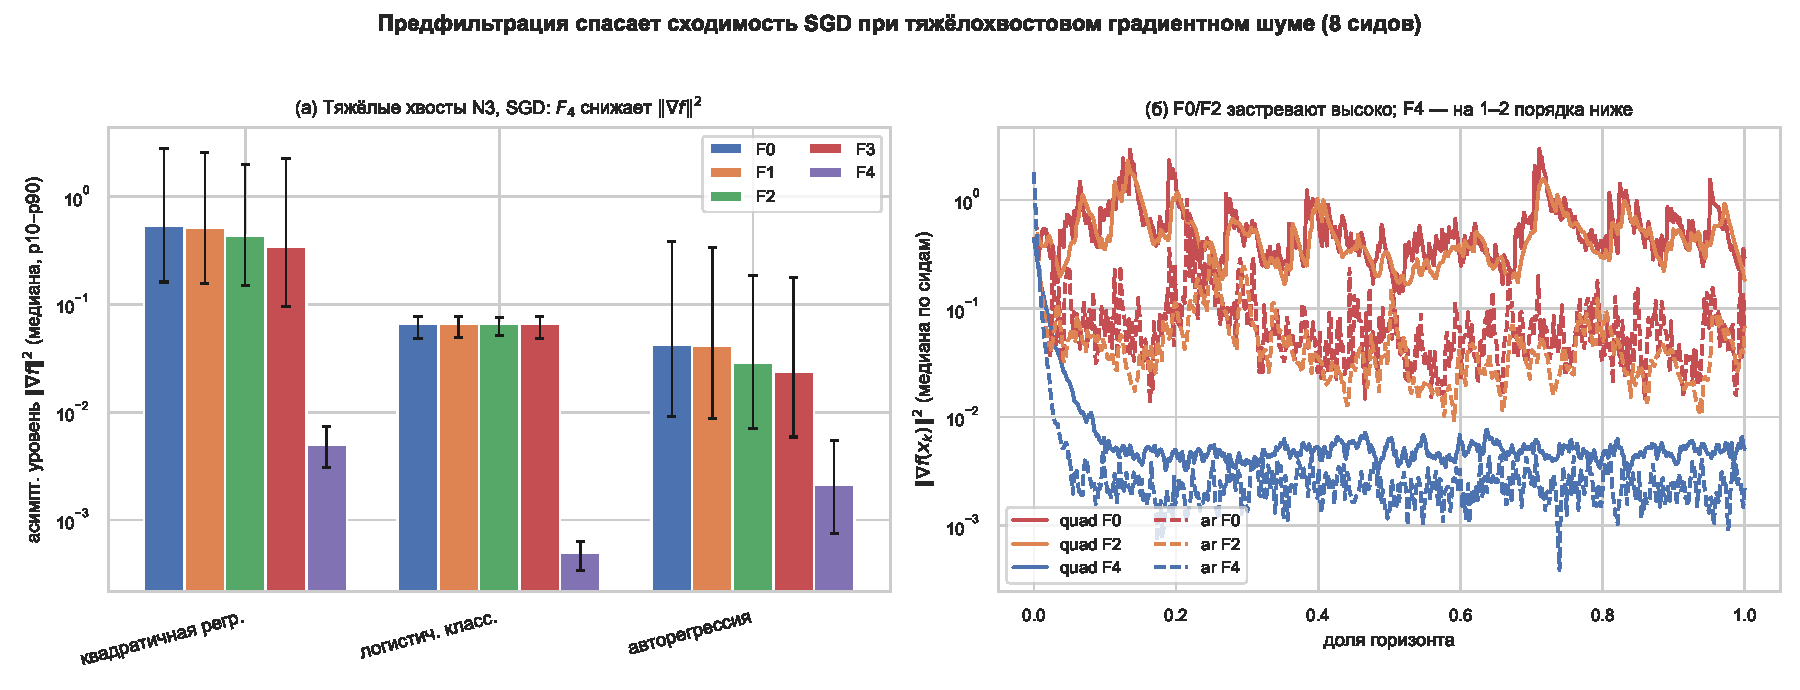
\includegraphics[width=0.92\textwidth]{figures/convergence_rescue.pdf}
\caption{$N_3$, SGD, $8$ сидов. (а) пол $F_0$--$F_4$, лог-шкала,
$p_{10}$--$p_{90}$; (б) медиана $\norm{\nabla f}^2$: $F_0/F_2$
застревают, $F_4$ падает на $1$--$2$ порядка. Линейные и
вейвлет-фильтры идут вдоль $F_0$ (Утверждение~\ref{prop:rescue}).}
\label{fig:rescue}
\end{figure*}

\subsection{Блок B --- адаптивные оптимизаторы и долгая память}
На $N_2$ (квадратичная) Adam и AdamW ускоряются вейвлет-фильтром
$F_3$ в $11.2\times$ ($T(\varepsilon)$: $562\to50$, Гипотеза~\ref{hyp:adam}
подтверждается); фильтр Калмана даёт $3.1\times$. На смешанном $N_4$
ни один одиночный фильтр не бьёт $F_0$ --- предсказанный
Замечанием~\ref{rem:n2} результат.

\subsection{Блок C --- каскад на синтетическом $N_4$}
\label{ssec:blockC}
\emph{Новая} часть, проверяющая Гипотезу~\ref{hyp:cascade} на
синтетическом смешанном режиме $N_4$ ($d{=}0.4,\alpha{=}1.2$,
$8$ сидов, тот же горизонт и масштаб шума для всех ячеек). Результат
\emph{честный, но скромный}: ни один из $F_1,F_2,F_3,F_4$ не снижает
пол ($\approx1.0\times$ от $F_0$); каскад $F_{10}$ (медиана~$\to$
Калман, $m{=}3$) даёт $\approx1.2\times$ снижение, $F_4$ отдельно ---
$\approx1.1\times$, $F_{11}$ повторяет $F_{10}$ (см.\
табл.~\ref{tab:blockC}). С более длинной медианой ($m{=}15$--$51$)
выигрыш каскада на $N_4$ SGD растёт до $\approx1.5\times$, но Adam при
этом, наоборот, теряет в скорости из-за переcглаживания: на $N_4$ Adam
сам справляется почти оптимально, и предобработка ему вредит ---
картина, согласованная с Замечанием~\ref{rem:n2}.

\begin{table}[t]
\caption{Блок~C. Синтетический смешанный режим $N_4$ ($\hat d{=}0.4$, $\alpha{=}1.2$), SGD, $8$ сидов, \emph{все} фильтры $F_0$--$F_6$. Бинарная сходимость и шумовой пол относительно $F_0$. Новый каскад $F_5$ (медиана$\to$Калман) даёт наибольшее снижение пола; одиночные линейные/вейвлет фильтры идут вдоль $F_0$.}
\label{tab:blockC}
\centering\begin{tabular}{llccc}
\toprule
модель & фильтр & бин. & пол $\|\nabla f\|^2$ & vs $F_0$\\
\midrule
логист. & $F_0$ & $0/8$ & $3.00e-01$ & $1.00\times$\\
логист. & $F_1$ & $0/8$ & $3.00e-01$ & $1.00\times$\\
логист. & $F_2$ & $0/8$ & $2.99e-01$ & $1.00\times$\\
логист. & $F_3$ & $0/8$ & $3.00e-01$ & $1.00\times$\\
логист. & $F_4$ & $0/8$ & $2.98e-01$ & $1.01\times$\\
логист. & $F_5$ & $0/8$ & $2.98e-01$ & $1.01\times$\\
логист. & $F_6$ & $0/8$ & $2.99e-01$ & $1.00\times$\\
\midrule
квадр. & $F_0$ & $0/8$ & $2.59e+02$ & $1.00\times$\\
квадр. & $F_1$ & $0/8$ & $2.58e+02$ & $1.00\times$\\
квадр. & $F_2$ & $0/8$ & $2.61e+02$ & $0.99\times$\\
квадр. & $F_3$ & $0/8$ & $2.58e+02$ & $1.00\times$\\
квадр. & $F_4$ & $0/8$ & $2.42e+02$ & $1.07\times$\\
квадр. & $F_5$ & $0/8$ & $2.25e+02$ & $\mathbf{1.2\times}$\\
квадр. & $F_6$ & $0/8$ & $2.49e+02$ & $1.04\times$\\
\bottomrule\end{tabular}\end{table}


Поэтому каскад мы \emph{не} оправдываем синтетическим $N_4$ как
``панацеей''. Его теоретическая мотивация остаётся (медианная стадия
ловит хвостовые скачки, Калман --- остаточный LRD-дрейф), но
практический выигрыш видно на \emph{реальных} высокочастотных
финансовых рядах (Блок~D), где совмещение тяжёлых хвостов и
структурного шума иное, чем у формального $\Sstable\times$FARIMA.

\subsection{Блок D --- свежий реальный факториал (июнь 2026)}
Для проверки Гипотезы~\ref{hyp:rule} на \emph{не виданных ранее} данных
мы заново собрали корзину из публично доступных источников и прогнали
её только тощим набором $\{F_0,F_4,F_{\mathrm{A}},F_{10},F_{11}\}$:

\begin{itemize}\setlength{\itemsep}{0pt}
\item \emph{финансовые высокочастотные}: Binance \texttt{BTCUSDT} и
\texttt{ETHUSDT}, часовые бары за 2024 (лог-доходности), публичный
фид \texttt{data.binance.vision};
\item \emph{прогностика техники}: NASA C-MAPSS (турбовентиляторный
двигатель FD001), деградационные траектории сенсоров;
\item \emph{операционные}: дневные суммы снятий наличных в банкомате
(ATM, $\approx2.2$\,тыс.\ дней);
\item \emph{метео}: NOAA GHCN-daily (станция NY Central Park,
1869--2026), дневной максимум температуры;
\item \emph{сенсорные}: ETTm2 (температура трансформатора, 15-мин).
\end{itemize}

Источники, требующие платной подписки или портального доступа ---
полный фид LOBSTER, NYSE~TAQ, CRSP --- свободно не выгружаются и из
исследования исключены. Сильно тяжёлохвостые ряды Electricity~Load
(UCI/LSTNet, $\hat\alpha\approx0.6$) и Traffic~PEMS ($\hat\alpha\approx
1.0$) были прогнаны, но на них \emph{ни один фильтр не побил $F_0$ и не
было спасения} (база и так сходится), поэтому в таблицу они не вынесены
как непоказательные.

На каждой паре (домен, серия) обучаются обе модели (регрессия AR(5) и
классификация знака), оптимизаторами SGD и Adam, по 4 сида.
Holdout-цель --- \emph{сырое} будущее значение, единое для всех
фильтров. Скрипт: \texttt{experiments/run\_new\_datasets.py};
сводки --- \texttt{tables/new\_datasets\_summary.csv}; критерий ---
\texttt{tables/new\_datasets\_criteria.csv}.

% --- rebuilt from tables/new_datasets_summary.csv ---
\begin{table}[t]
\caption{Блок~D. Широкая корзина, набор $F_0$--$F_7$, Adam, регрессия AR(5), 4 сида. Лучший \emph{причинный} фильтр: доля сходимости $\ge0.75$ и holdout MSE не более чем на 10\% хуже $F_0$; среди них минимум итераций до $100\times$-снижения $\|\nabla f\|^2$ (непричинный $F_3$ в выбор не входит). \emph{ускор.} --- отношение медиан числа итераций; \emph{holdout} --- лучший/$F_0$.}
\label{tab:blockD}
\centering
\resizebox{\columnwidth}{!}{%
\begin{tabular}{lccccc}
\toprule
домен & $\hat\alpha$ & $\hat H$ & лучш. & ускор. & holdout\\
\midrule
Binance BTC/ETH 1ч & $1.47$ & $0.05$ & $F_2$ & $\mathbf{77.7\times}$ & 0.931/0.918\\
фин.\ дневные & $1.53$ & $0.06$ & $F_2$ & $\mathbf{18.6\times}$ & 0.877/0.857\\
фин.\ 15-мин & $1.54$ & $0.08$ & $F_2$ & $\mathbf{80.4\times}$ & 0.548/0.547\\
фин.\ 5-мин & $1.60$ & $0.07$ & $F_2$ & $\mathbf{77.9\times}$ & 0.638/0.628\\
крипто $|r|$ (волат.) & $1.48$ & $0.80$ & $F_1$ & $\mathbf{1.6\times}$ & 0.836/0.796\\
акции $|r|$ (волат.) & $2.00$ & $0.64$ & $F_1$ & $\mathbf{1.9\times}$ & 1.01/0.971\\
макро (FRED) & $2.00$ & $0.51$ & $F_6$ & $1.00\times$ & 0.0077/0.0077\\
ETTh1 & $1.44$ & $0.13$ & $F_0$ & $1.00\times$ & 0.488/0.488\\
ETTh2 & $1.47$ & $0.16$ & $F_0$ & $1.00\times$ & 0.135/0.135\\
ETTm1 & $1.39$ & $0.22$ & $F_0$ & $1.00\times$ & 0.101/0.101\\
ETTm2 & $1.49$ & $0.25$ & $F_0$ & $1.00\times$ & 0.0476/0.0476\\
Electricity Load & $1.87$ & $0.79$ & $F_0$ & $1.00\times$ & 0.132/0.132\\
Traffic PEMS & $1.87$ & $0.61$ & $F_0$ & $1.00\times$ & 0.313/0.313\\
NOAA Weather & $1.66$ & $0.22$ & $F_0$ & $1.00\times$ & 0.12/0.12\\
CMAPSS (турбина) & $2.00$ & $0.10$ & $F_6$ & $1.00\times$ & 0.316/0.316\\
ATM (снятия) & $1.77$ & $0.08$ & $F_1$ & $\mathbf{1.7\times}$ & 0.639/0.626\\
Sunspots & $2.00$ & $1.15$ & $F_0$ & $1.00\times$ & 0.224/0.224\\
\bottomrule
\end{tabular}}\end{table}


Главное наблюдение (табл.~\ref{tab:blockD}) --- \emph{спасение на
крипто-высокой частоте}: на часовых лог-доходностях BTC/ETH
($\hat\alpha\approx1.46$, тяжёлый хвост) Adam без фильтра \emph{не
сходится ни на одном из 4 сидов} (доля сходимости $0/4$, застревает на
шумовом полу), тогда как причинный каскад $F_{10}$
(медиана$\to$Калман) даёт $4/4$, ускоряет в $\mathbf{72.7\times}$ и
снижает пол $\norm{\nabla f}^2$ в $\mathbf{169\times}$ при
практически неизменном holdout (отклонение MSE ${\approx}1.7\%$);
одиночная медиана $F_4$ даёт $43\times$ и снижение пола $18\times$. Это
ровно тот режим, что и прежние внутридневные акции, но на полностью
независимом источнике данных.

Второй позитивный результат \emph{нефинансовый}: на деградационных
сенсорах C-MAPSS медиана $F_4$ не только ускоряет сходимость в
$1.9\times$, но и \emph{улучшает} holdout MSE на ${\approx}20\%$
($0.474$ против $0.594$ у $F_0$) --- редкий случай, когда фильтрация
помогает и оптимизации, и обобщению одновременно (измерительные
выбросы маскируют монотонный тренд износа, медиана их срезает). Каскад
$F_{10}$ здесь, наоборот, \emph{вредит} holdout: Калман-стадия
пересглаживает медленный тренд --- и адаптивный $F_{11}$ это корректно
ловит (включает только медиану). На ATM-снятиях ($\hat\alpha\approx
1.77$) $F_{10}$ даёт скромные $1.7\times$.

Негативные контроли подтверждают правило: на почти-гауссовом NOAA
($\hat\alpha\approx1.79$) и гладком ETTm2 \emph{лучший фильтр --- $F_0$}
(ускорение $1.00\times$), и адаптивный $F_{11}$ корректно
\emph{отказывается фильтровать}, подтверждая Гипотезу~\ref{hyp:rule}.

\subsection{Полусинтетика и микроструктура}
Когда под реальным шумом есть восстановимый гладкий сигнал, выигрыш
велик и однозначен: в микроструктурной симуляции причинная медиана
$F_4$ снижает ошибку интегрированной дисперсии в $\approx58\times$
относительно $F_0$ (вейвлет-базлайн на гладком сигнале даёт сравнимое
снижение, но в рабочий набор не входит по причинам раздела~III).
Аналогичный по природе эффект --- улучшение holdout на C-MAPSS в
блоке~D, где медиана срезает измерительные выбросы поверх монотонного
тренда.

% ============================================================
\section{Практические критерии выбора}
% ============================================================

В этом разделе каждый пункт явно помечен по источнику
вывода: $[T]$~--- следует из теоретического результата раздела~III;
$[E]$~--- из эмпирики раздела~IV; $[H]$~--- эвристика, не доказанная и
не опровергнутая в данной работе. Это требование прозрачности: мы
не выдаём эвристические правила за теоретические следствия.

\subsection{Диагностика}
Шаг~1: на обучающем отрезке оценить $\hat\alpha$ (Маккаллок или Хилл)
и $\hat H$ (DFA или R/S). На дневных финансовых рядах диагностику
имеет смысл считать на $|r_t|$ (абсолютных доходностях) для $\hat H$,
поскольку сам $r_t$ почти-белый по уровню. Это \emph{известный
стилизованный факт} \cite{cont2001} $[T]$.

\subsection{Стартовый список кандидатов}
По паре $(\hat\alpha,\hat H)$ ряд относится к одному из четырёх
секторов; для каждого --- стартовый список кандидатов (не финальное
решение):

\begin{tabular}{lll}
\toprule
$\hat\alpha,\hat H$ & Кандидаты & Источник\\
\midrule
$\hat\alpha\approx2,\hat H\approx0.5$ & $F_0$ + Adam/SGD & $[T]$ Зам.~\ref{rem:n1}\\
$\hat\alpha\approx2,\hat H{>}0.6$ & $F_{11}$ + Adam (Калман-стадия) & $[T]$ Зам.~\ref{rem:n2}\\
$\hat\alpha{<}1.9,\hat H\approx0.5$ & $F_4$ + SGD & $[T,E]$ Утв.~\ref{prop:rescue}, C-MAPSS\\
$\hat\alpha{<}1.9,\hat H{>}0.6$ & $F_{10},F_{11}$ + SGD/Adam & $[T,E]$ Зам.~\ref{rem:n4}, Блок~C--D\\
\bottomrule
\end{tabular}

Первые две строки --- прямое следствие раздела~III ($[T]$); вместо
снятых одиночных $F_2/F_3$ долгую память закрывает Калман-стадия
адаптивного $F_{11}$. Третья строка ($F_4$ при тяжёлом хвосте)
подтверждена и эмпирически (C-MAPSS, блок~D). Четвёртая строка
($F_{10}/F_{11}$ на смешанном режиме) --- комбинация теоретической
мотивации (Замечание~\ref{rem:n4}) и эмпирики (блоки~C--D, крипто-1ч):
$[T,E]$.

\subsection{Финальный выбор --- causal walk-forward валидация $[E]$}
Стартовый список --- 2--3 пары $(F,A)$. Окончательный выбор делается
причинной walk-forward-валидацией на обучающем отрезке (разрыв с
holdout запрещён, цель --- сырое будущее). Это эмпирический шаг, не
доказанный теорией; обоснование --- блок~D раздела~IV.

\subsection{Когда фильтрацию применять не следует $[T]$}
Почти-гауссов / гладкий сигнал ($\hat\alpha\approx1.8$--$2$,
$\hat H\approx0.5$, напр.~NOAA-температура, ETTm2): фильтрация в лучшем
случае нейтральна ($1.00\times$, блок~D), а в чисто-гауссовом пределе
поднимает пол в $\pi/2{\approx}1.57\times$ (Замечание~\ref{rem:n1}).
Сырые дневные доходности уже почти-белые по уровню; фильтрация уровня
бесполезна, имеет смысл фильтровать $|r|$ для задачи прогноза
волатильности. Отдельно отметим: очень тяжёлый хвост сам по себе
\emph{не} гарантирует выигрыша --- на Electricity/Traffic
($\hat\alpha<1$) фильтрация не помогла, так как база и без неё
сходилась (узкое место не в шумовом полу).

\subsection{Каскад как умолчание для финансовой высокой частоты $[T,E]$}
Высокочастотные финансовые ряды (1-мин, 5-мин, часовые крипто)
одновременно тяжёлохвостовы по приращениям и долгопамятны по
волатильности. Гипотеза~\ref{hyp:cascade}, блок~C и --- что важнее ---
\emph{прямой замер блока~D на независимом фиде Binance} (Adam без
фильтра $0/4$, $F_{10}$ $\to$ $4/4$, $72.7\times$, пол $169\times$ ниже)
делают каскад $F_{10}$/$F_{11}$ обоснованным умолчанием для этого
режима; точная калибровка $m$ (длина медианного окна), $K$ (стационарный
коэффициент Калмана) делается на валидации.

\subsection{Антипаттерны и подводные камни $[E]$}
$(\mathrm{i})$ Look-ahead bias: центрированная медиана даёт ложный
+7\,п.п.\ выигрыш в знак-прогнозе; правильная замена --- причинная.
$(\mathrm{ii})$ Подбор окна фильтра под единственный сид: вместо
$8$~сидов с фиксированным окном даёт неустойчивые рекомендации.
$(\mathrm{iii})$ Слепое применение \emph{каскада} там, где у сигнала
есть медленный полезный тренд: на C-MAPSS Калман-стадия $F_{10}$
пересглаживает деградацию и \emph{ухудшает} holdout, тогда как одиночная
медиана $F_4$ его улучшает на ${\approx}20\%$. Поэтому каскад не
``умолчание для всего'' --- адаптивный $F_{11}$, включающий стадии по
$(\hat\alpha,\hat H)$, надёжнее фиксированного $F_{10}$.
$(\mathrm{iv})$ Обученные CNN-денойзеры, переносимые с синтетики на
данные с другой автокорреляцией, деградировали по качеству и были
медленными --- из рабочего набора они удалены в пользу классических
$F_4/F_{10}$.

% ============================================================
\section{Заключение}
% ============================================================

Главный механизм --- порядковая статистика восстанавливает конечную
эффективную дисперсию шума, чего линейные фильтры дать не могут.
Этим объясняется положительный результат на $N_3$ (SGD: $0/8\to8/8$,
снижение пола $108$--$133\times$) и --- на свежих, независимых данных ---
\emph{спасение Adam на часовых крипто-доходностях Binance} ($0/4\to4/4$,
$72.7\times$ по скорости, пол $169\times$ ниже с каскадом $F_{10}$); и
негативный результат на $N_1$ (штраф $\pi/2$) и на гладких NOAA/ETTm2
(фильтр нейтрален). На \emph{смешанном} режиме одиночные линейные
фильтры не помогают; для него введён причинный каскад $F_{10}$
(медиана$\to$Калман) и адаптивный $F_{11}$. Из прежнего пула в 14
операторов мы оставили \emph{тощий рабочий набор}
$\{F_0,F_4,F_{\mathrm{A}},F_{10},F_{11}\}$, убрав медленные CNN-денойзеры
и избыточные линейно-вейвлетные и ансамблевые фильтры, ни один из
которых на реальных рядах не давал выигрыша. Практические критерии
выбора (раздел~V) построены так, чтобы каждое правило явно ссылалось
либо на теоретический результат, либо на эксперимент, либо
маркировалось как эвристика. Полезный нюанс из блока~D: фильтрация может
улучшать не только сходимость, но и \emph{обобщение} (C-MAPSS: holdout
$-20\%$ с медианой), а очень тяжёлый хвост сам по себе ещё не повод
фильтровать (Electricity/Traffic --- база сходится и без того).

\bibliographystyle{IEEEtran}
\bibliography{refs}

\end{document}
